\documentclass{article}
\usepackage[utf8]{inputenc}
\usepackage[english]{babel}
\usepackage{graphicx}

\title{CSE344 FINAL PROJECT}
\author{Can Beyaznar - 161044038}
\date{June 2020}

\usepackage{natbib}
\usepackage{graphicx}

\begin{document}

\maketitle

\section{Problem Solution}
\subsection{Server Part}

First of all, I checked the values of inputs from the user with the help of getopt in the server part. If it does not comply with the rules specified in the homework, I print the usages to the terminal and end the program. If it's correct, I'm doing a check to prevent the server from running again. For this, I check the file named 
$"$ \texttt{\_ISSERVER\_WORKING\_} $"$ 
with the access () function. If this file already existed, the server is running. If this file does not exist, I create the file with the fopen () function. Thus, if the server is run again, I prevent multiple servers from running at the same time. And I definitely delete this file at the end of the program. Important note, if, under any error condition, the file 
$"$ \texttt{\_ISSERVER\_WORKING\_} $"$ 
has not been deleted, please delete this file, otherwise the server will not work.
\newline
And now I can allocate global values that I will use on my server. I do this in the \texttt{prepare\_server} section. Here, for my 2D array named myGraph, I need to determine the size and fill it in. First of all, I read the file entered by the user and find the maximum NodeID in the file. I also terminate the program if there is any mistake in the file entered by the user. These inaccuracies include negative numbers, TAB (ascii value: 9) between two numbers, and space instead. \textbf{There must be a TAB between the two numbers or the program will not run.}  After learning the maximum NodeID, I create an array named \texttt{EdgeSize\_EachNode}. This array is size up to NodeID + 1. In this array, I count how many nodes each node points to. After this process, I now learn the size I need to reserve for my 2D graph array. The structure of my graph is as follows.


\begin{center}
    \centering
    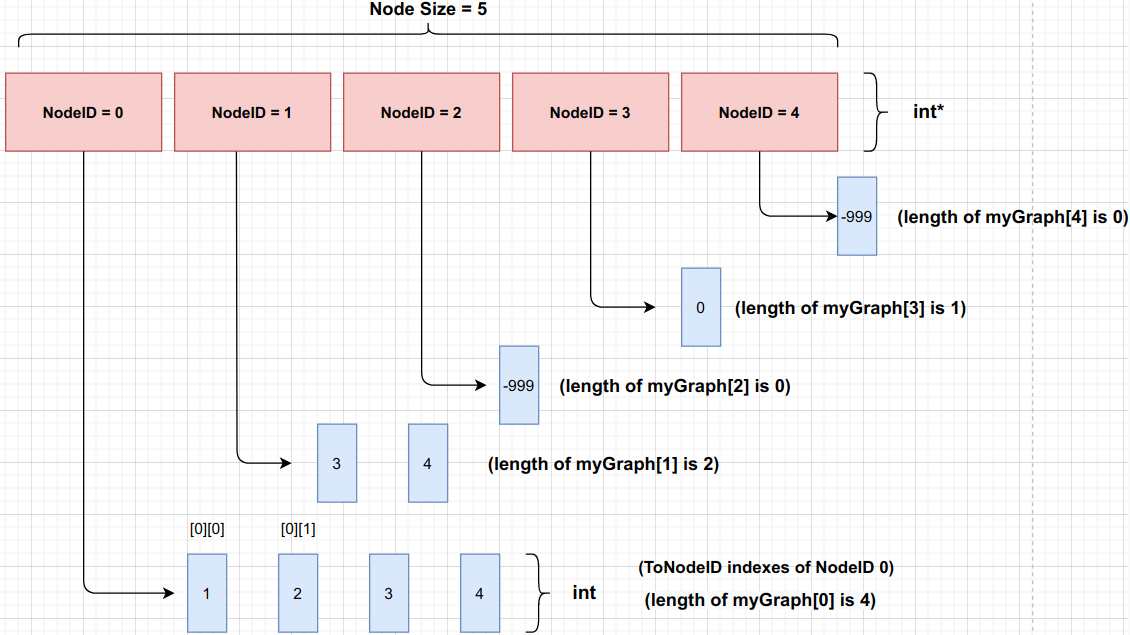
\includegraphics[scale=0.5]{img1.png}
    2D Graph Structure
     \label{fig:myGraph}
     
    
\end{center}
\begin{center}
    \centering
    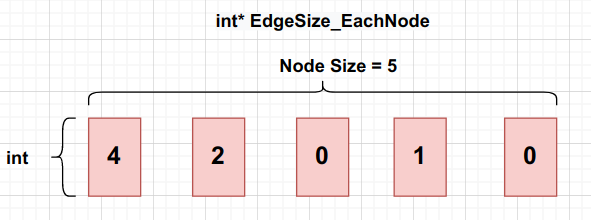
\includegraphics[scale=0.5]{img2.png}
    \newline\texttt{EdgeSize\_EachNode Array}
    \label{fig:myGraph}
\end{center}


After reserving a place for Graph, I re-read the file to fill in the information. Assigns the ToNodeID to the current index by going to the index of FromNodeID read from the file. Thus, our graph becomes completely ready. Then, space is reserved for the parameters required for the threads. In this assignment, I used pipes to facilitate communication between main and thread. There will be a total number of threads in total and these pipes will be updated as they are resized. The \texttt{socket\_fd} sent by the main using the pipe in the threads is received by the thread in sequence and no requests remain unanswered. After this process, I initialize the mutex that I will use for threads according to \texttt{priority\_type}. Then my reservation is finished.
\newline
\newline
After these processes, I create my threads. I created the \texttt{thread\_inf} structure to solve problems such as f finding the available thread, learning the id of the thread. And I created a structre named \texttt{thread\_list} to keep them connected. \texttt{thread\_list} structure is a linked list that holds \texttt{thread\_inf} values. I send my threads to my parameter \texttt{thread\_pool} of \texttt{thread\_list} type. After creating threads, I can now switch to the socket creation section. After opening the socket in \texttt{AF\_INET} type, I am waiting for a request from the client with accept (). After the request, I first check the server load, if it is over 75, I send a character to my resize thread using pipe. When Resize reads this character, it has two options. If the character is 'r', it resizes, if 'e' exits and ends the thread. A similar process is available in the thread calculating BFS. After resizing, the find thread is checked by calling the findAvailableThread () function. Here the int isRunning parameter in my \texttt{thread\_inf} structure comes into play. If this parameter is 0, it means available, if it is 1, it means busy. The findAvailableThread function returns the index of the thread where it sees the first 1 value. If they are all full, they wait. Then \texttt{socket\_fd} is sent to the pipe of the thread that should work. And when the threads are running, it takes the file descriptor from its pipe and calculates according to the source and destination sent by the Client. In addition, in order to end my threads calculating BFS, I provide their output by sending -1 to the values sent by pipe. Also, when creating each thread, I send the information of \texttt{thread\_inf} type as a parameter. Thus, this information can be updated in the thread. And in main I can find out which threads are busy or available. The structure I created for the thread pool is as follows.

\begin{center}
    \centering
    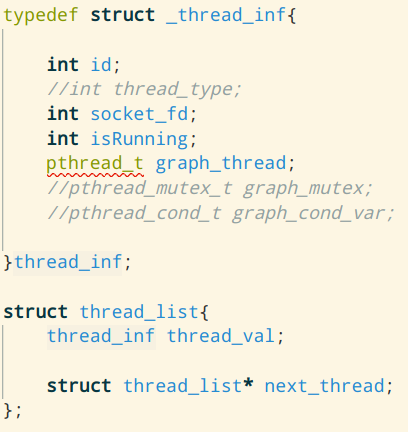
\includegraphics[scale=0.5]{threadpool.png}
    
    \label{fig:myGraph}
\end{center}


If we come to the thread function calculating BFS. First of all, I read the values from the main pipe. If all values are -1, the thread terminates itself. If not, I am reading \texttt{socket\_fd} from main. And I define the char array I will send to the client. I allocated the size of this array as (char *) malloc (sizeof (char) * 40960). However, if the path from BFS is longer than this, the client will definitely not get the correct result of the path. Therefore, please run the program with this problem in mind. Since no value can be sent according to the length of the path to be sent in the sockets, a fixed size has been determined by compelling. With this dimension, a path can contain an average of 5120 numbers in itself. After the reservation, we use our mutex according to the \texttt{priority\_type} value from the user. The same algorithm is used in 3 possibilities. The only difference is the way mutex is used and the way it is used. While writing these algorithms, the reader writer problem's algorithm described in the lesson was used. If we come to the path finding algorithm, firstly, the source and destination values are taken by the client with the recv () function. Then, it is checked whether this path is available in the Cache database (Cache structure will be explained later). If not, the path is calculated with BFS and written to the log file and added to the Cache database. If there is no way, an error is given.
\newline
\newline

Coming to the cache structure, I chose the Binary Search Tree structure to make the searches faster here. I thought that this structure is more suitable because I will use only search and insert in the database. Since it has search and insert {log n} time complexity, I think I can add and remove database quickly. The structure I created for the cache database is as follows.
\begin{center}
    \centering
    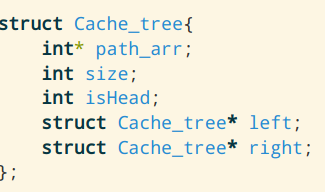
\includegraphics[scale=0.5]{cachetree.png}
    
    \label{fig:myGraph}
\end{center}
If we come to the resize thread, first of all, I read the character coming from main with the help of pipe. If it is 'e', I exit, if 'r', I resize. Before calculating, I calculate how many threads I need to create. If 25\% of the current thread count is 0, I create 1 new thread. So I prevent my resize thread from working in vain. Then I create threads as many threads as they need to create.
\newline
I keep a parameter for the \textbf{SIGINT} signal like I did in previous assignments. When \textbf{SIGINT} occurs, I set the value of this parameter to 1. And I can end my program by checking this value in \textbf{non-critical} areas of my program.

\subsection{Client Part}
The client part is simpler than the server part. First of all, I get the inputs that I need to get from the user with getopt and check these values. Source and destination must be positive. After these checks, I contact the server. Then I send the source and destination that should be sent to the server with the help of send. Then I wait for the response from the server with the recv function. As I mentioned in the server part, I got the size of the answer here as much as 40960. Thus, if the answers do not exceed this limit, the path reaches the client's hand correctly. The result is printed on the screen according to the response.

\subsection{Example Output}
\begin{center}
    \centering
    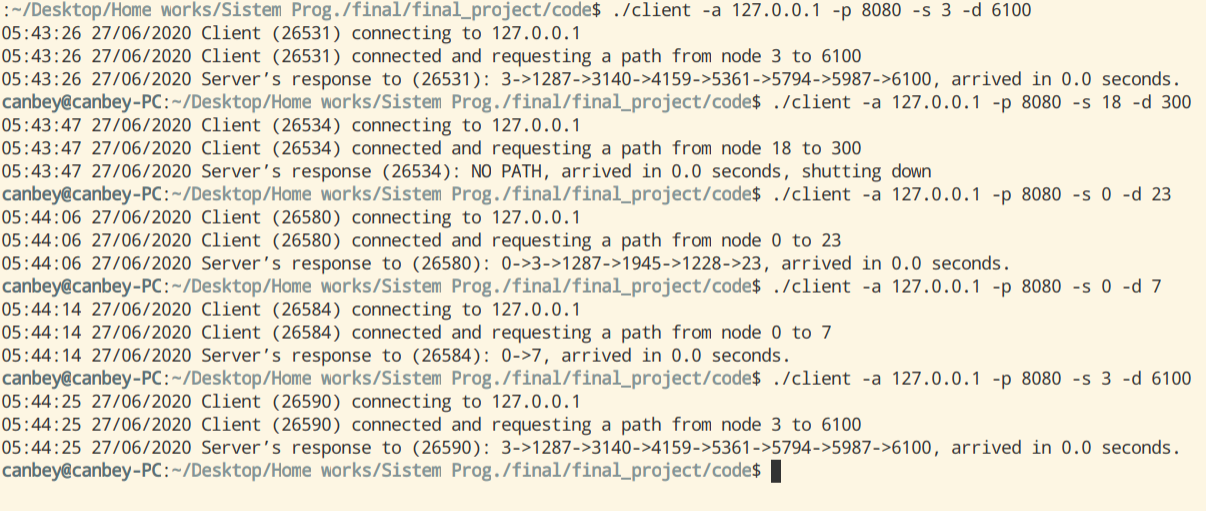
\includegraphics[scale=0.5]{img3.png}
    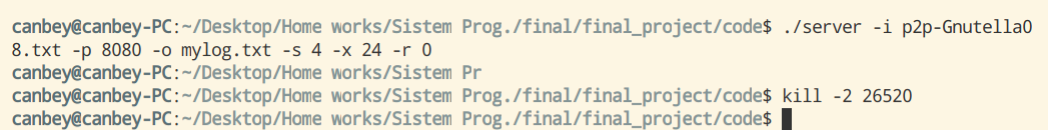
\includegraphics[scale=0.5]{img5.png}
    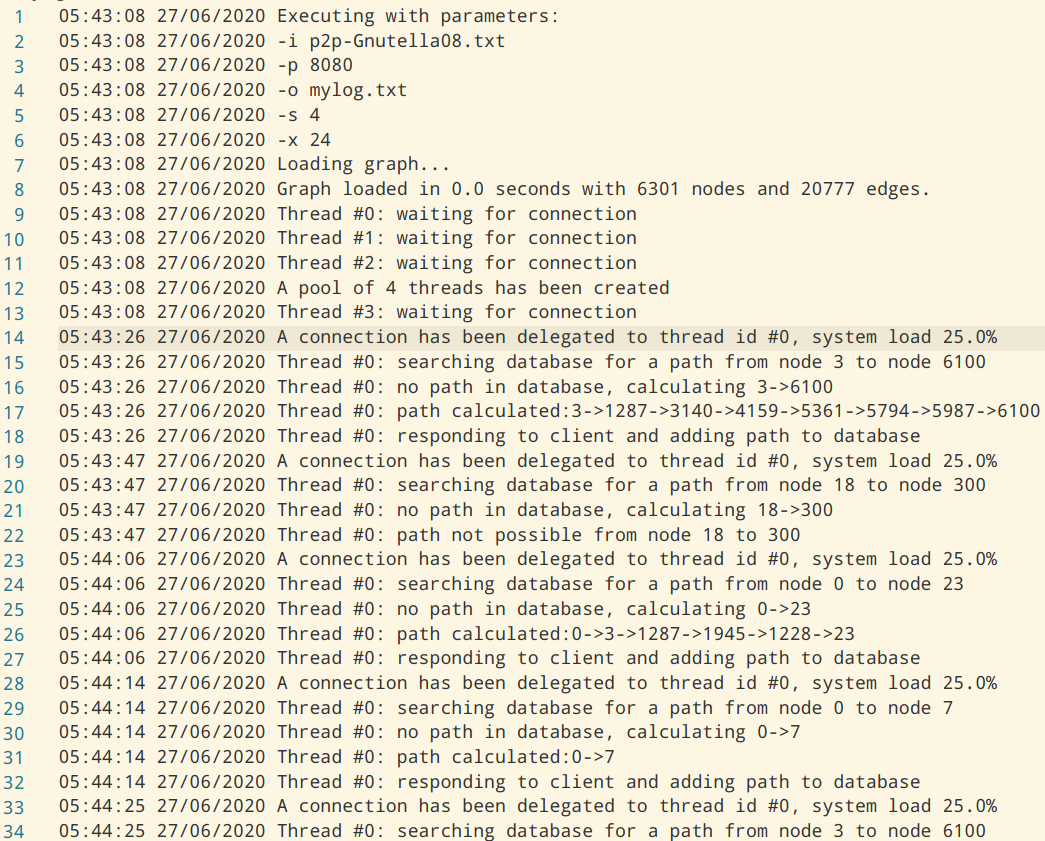
\includegraphics[scale=0.5]{img4.png}
    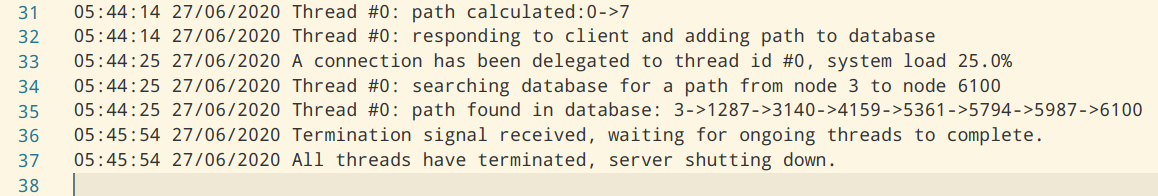
\includegraphics[scale=0.5]{img6.png}
    
    \label{fig:myGraph}
\end{center}
\subsection{Important Notes}
NodeIDs should not be negative.
\newline
The server program should always be run in the same location. (To check \texttt{\_ISSERVER\_WORKING\_} file)
\newline
There must be TAB between 2 NodeIDs.

\end{document}
